
\section{Application Payloads}

While the amount of computation done in a single speculative execution is small,
we demonstrate several applications that can take advantage of multiple
speculative runs to carry out computation.

As a first step, we observe that this primitive can be used to trivially
implement a finite state machine: any logic can be done in the speculative
world, while updates to the state are communicated to the real world where they
are stored. On the next run of the speculative instructions, they read from the
real world state (and other inputs), compute any state transitions, and
communicate the result. In this mode, the state is maintained by the real world,
while updates are controlled by code executed speculatively.

Next, we observe that the instructions to be executed speculatively can be
obscured further by encrypting them. This encryption allows for hidden
computation, instructions are stored in the real world encrypted, they are then
decrypted in the speculative world and passed to the real world to be executed.
This method makes it appear as though the program is generating its own code.

\begin{figure}[t]
    \centering
        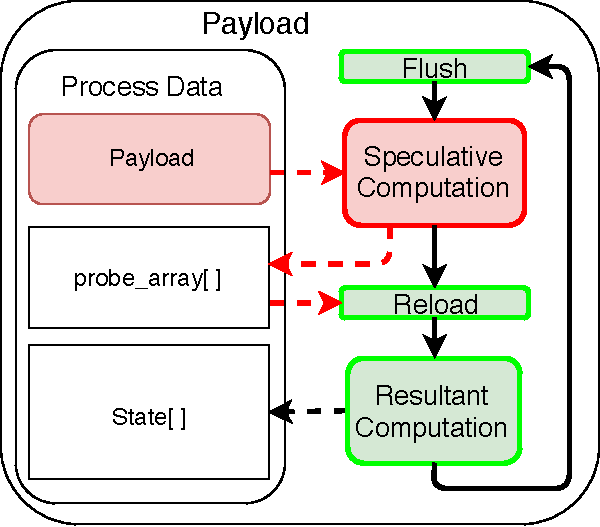
\includegraphics[width=0.4\textwidth]{figures/general_model}
    \caption{ General model of speculative computation within the Measure 
        process when triggered. \textit{Speculative Computation} has access
        to all variables which do not require a memory transaction within
        the current state of the process. The process can subsequently make
        \textit{Resultant Computations} based on the value returned from 
        Prime and Probe to update the state of the process. }
    \label{fig:general_model}
\end{figure}


\subsection{Turing Machine}
\label{subsec:turing}
To demonstrate that arbitrary computation can be done in the speculative world
we create a Turing Machine to compute a 6 state Busy Beaver Turing Machine. 

\subsection{Unpacking and Decryption}
\label{subsec:decryption}
While Section \ref{subsec:turing} demonstrates that arbitrary computation is
possible, if a reverse engineer can discover the \emph{speculative instructions}
they can determine the execution of the program by simply reading the
instructions that are to be executed speculatively. To avoid this these
instructions can be encrypted, meaning that a reverse engineer can never
determine these instructions by examining the ELF file, or generating source
code. 

In order for these instructions to be executed they must be decrypted. We wish
to obscure the fact that we are using encrypted instructions from the ``real
world'', thus  the speculative world must do the decryption. 

Any observer watching the execution of this program would never see any
indication of decryption, due to the exploitation of speculative execution. Any
observation of the executed instructions would not include any of the decryption
instructions, or loading of keys as they are only done speculatively, and thus
not shown in any debugging or real world traces of program execution.
Additionally the observer would be unable to find the executed instructions in
the ELF file as they are only stored encrypted. 

There are numerous challenges for a reverse engineer to overcome to learn how a
malicious program with this primitive works. As with previous examples, the
malicious instructions are only executed when the correct trigger program is
running (priming the jump table predictor \textbf{TK: word for this?}). However,
when the to-be-executed instructions are executed the reverse engineer cannot
locate these instructions in the ELF file, or generated source code. These
instructions (when they even appear) seem to be generated by themselves, with no
apparent cause. Additionally, there is no indicator that these instructions are
encrypted as the decryption is done in the speculative world, meaning that no
decryption (or key interaction) is done in a way visible to a reverse engineer.

This method allows for arbitrary computation that is unobservable to any observer (static or dynamic). 


% 
% Argument for obfuscating keyschedule
% 
% Challenge for Rev-Engineer
%   - Find the obfuscated key schedule
%   - Find the correct trigger program

\subsection{Virtual Machines}
Given the specific constraints that the speculative environment enforces on
these payloads, general purpose computation []. We demonstrated in
Section~\ref{subsec:turing} that general purpose computation is possible using
computation performed in the speculative environment. However, a turing machine
is not a user friendly model, nor is it an efficient model for computation when
attempting to accomplish tasks on modern processors. 

Using emulators in the "real world" allows for crafted binary programs to be
instrumented in dead code and, as demonstrated in
Section~\ref{subsec:decryption} encrypted and hidden. This gives an advantage to
attackers as traditional reverse engineering methods will reveal only that
emulation is being done. It reveals nothing about the ultimate goal of the
program. 

To accomodate both developers as well as the unique constraints 
enforced by the speculative primitive, a custom emulation solution is required. We 
have approached this challenge from both directions. First we demonstrate 
general purpose emulation using a custom instruction set -- SPASM -- which
accomodates the speculative primitive specifically. Next we investigate custom 
wrappers on traditional emulators allow for similar payload construction,
with a much more developer friendly 

% REFERENCE FIGURES
% - Constraints enforced by speculative primitive
%       - more bits = slower
%       - less bits = less expressive
%       - must be computable within speculative ROB limit (~150 instrs) (decrypt only)
%   
% - optimizations for weird-machine computations 

% --- VM
%   - Wrappers around traditional ISA VMs
%   - SPASM  custom emulator made f
%%%%%%%%%%%%%%
